chapter2 notes

	%\item Extend the current lead time of predictability further back in time, into the December preceding the summer storm season
	%\item Create a statistical model that can be used as a benchmark for dynamical models, namely the Met Office's GloSea5
	
%The peak season for tropical storm activity in the West Pacific is boreal summer, and so the months of June-October inclusive were chosen. %occurring within these four months. Say what seasonality is based-wide, then show the plot in the method or results, where look at ACE and counts in my region ACE Is.... correlates with damage better than frequency

%This region because latitudinal difference in China landfalls primarily ENSO. Remove this change. Where population is including when cause damage further inland rather than just at point of landfall.

%I NEED TO CALCULATE LANDFALL PROBABILITY MAPS / HISTOGRAMS
%Using landfall probability maps (ref maps), based on JTWC data for JJAS storms 1970-2014, the domain was selected. The domain encompasses the region of highest landfall probability.... The number of storms .... Show a map of the storms.

%aCE index to cateogorise a season as normal, above normal or below normal, usually in combination with storm numbers (noaa web). Accumulated cyclone energy (ACE) is a measure used by the National Oceanic and Atmospheric Administration (NOAA) to express the activity of individual tropical cyclones and entire tropical cyclone seasons, particularly the Atlantic hurricane seasons. It uses an approximation of the energy used by a tropical system over its lifetime and is calculated every six-hour period.  Kinetic energy is proportional to the square of velocity, and by adding together the energy per some interval of time, the accumulated energy is found. As the duration of a storm increases, more values are summed and the ACE also increases such that longer-duration storms may accumulate a larger ACE than more-powerful storms of lesser duration.
%Although ACE is a value proportional to the energy of the system, it is not a direct calculation of energy (the mass of the moved air and therefore the size of the storm would show up in a real energy calculation).

%The spatial domain for analysis of SLP and SST is 40E to 120W (40-240). The domain for the TCHP is 40E to 80W (40-280). March-May seasonal means are used for these large-scale variables. 


%Can test for significant association by testing whether the population correlation is zero which is identical to the t-test used to test whether the population r is zero; d.f.=$n-2$. Use probability calculator for t distribution to get p-value (2-tailed if interested in association in either direction)1-tailed test for a positive correlation between x and y
%Proportional means linearly related; that is, the correlation is high if it can be approximated by a straight line (sloped upwards or downwards). This line is called the regression line or least squares line, because it is determined such that the sum of the squared distances of all the data points from the line is the lowest possible. 
%Within each box of high correlation, a mean value of the reanalysis variable is calculated. This annual value is correlated with the annual ACE value, to examine which relationships are strongest to give one statistic for correlation for each region identified.
%\beq
%t = \frac{r\sqrt{n-2}}{\sqrt{1-r^{2}}}
%\eeq

%Correlation maps of Pearson R value between the large-scale variables and ACE-JJASO are created. Based on these correlation maps and understanding of the physical processes that affect typhoon activity, regions of high correlation were selected. 
%\subsection{Statistical model}
%Stepwise regression is a systematic method for adding and removing terms from a linear model based on their statistical significance in explaining the response variable. The method begins with an initial model, and then compares the explanatory power of incrementally larger and smaller models. MATLAB® uses forward and backward stepwise regression to determine a final model. At each step, the method searches for terms to add to or remove from the model. The criterion selected is 'sse' and in this case, stepwiselm uses the p-value of an F-statistic to test models with and without a potential term at each step.
%Stepwise regression used and is a systematic method for adding and removing terms from a linear model based on their statistical significance in explaining the response variable. The ‘stepwiselm’ function in Matlab uses forward and backward stepwise regression to determine a final model. At each step, the method searches for terms to add to or remove from the model. For each variable, the mean value within each selected region for each season is fed into the model as a predictor, with the ACE-JJASO as the predictand. Only 50 years of data is used to create the model (1958-2007), with 7 years remaining to test (2008-2014).

%The forecast ability of the multivariate regression model is assessed using leave-one-out cross validation (LOOCV). 

%There is a strong seasonal cycle to the tropical storm activity within the specified domain (figure 2.2) and the pattern of ACE closely follows that of tropical storm frequency, with the peak around July, August and September, with approximately 1.6 storms per year when the value shown is divided by 57 years.

%\begin{figure}[h]
%	\noindent\includegraphics[width=16pc,angle=0]{Y:/Code_Data/Plots_folders/Plots_NCAR/Charts/seasons.png}\\
%	\caption{Tropical storm seasonal activity with the domain. Cumulative over all 57 years and ACE just for portion of storm within domain.}\label{fLOOCV}
%\end{figure}

%\begin{figure}[h]
%	\centering
%	\subfloat[a]{\includegraphics[width=16pc,angle=0]{Y:/Code_Data/Plots_112/Charts/count_intensity.png}} 
%	\subfloat[b]{\includegraphics[width=16pc,angle=0]{Y:/Code_Data/Plots_112/Charts/count_intensity.png}

%	\caption{Time series of storm frequency for different intensity categories.} 
%	\label{fig:EcUND} 
%\end{figure} 

%These initial results have shown various correlations, although with limited evidence of physical mechanisms.
%The remaining work on this study is to examine what are the drivers of these correlations and their predictability. I will examine relationships with atmospheric variables, which should provide information on the air-sea interactions.

%I will examine SST correlations with ACE-JJASO for the 12 months preceding the season, as some El Nino precursors may be apparent at this lead time.

%Look at area-averaged time series, ie. scatter plots
%Monthly activity?

%The primary driver of basin-wide ACE is El Ni\~{n}o, so .....how does this relate to El Ni\~{n}o effect in the specified domain.
%The results show that the frequency of storms affecting the domain is closely related to SST. This may be due to the genesis location of these storms or the storm track being favourable. The SST correlations with the basin-wide ACE are presented, to aid interpretation of these results.


%Look at the basin-wide ACE, to see whether this has an impact across the whole basin or just in the landfall domain interested in. Weak storms are remarkably similar when look at basin-wide ACE and count. Medium show similar weak correlations. Most intense storms show some differences, but still a significant negative correlation in the SCS (much weaker, although still significant)  (\ref{fig:corr_prevJFM_basin}).
%
%\begin{figure}
%	\centering
%	\subfloat[a]{\includegraphics[width=2.4in]{Y:/Code_Data/Plots_new/Corr_maps/ACE/basin/prev_sst_JFM&ACEJJASO63basincorr_train.png}} 
%	\subfloat[d]{\includegraphics[width=2.4in]{Y:/Code_Data/Plots_new/Corr_maps/count/basin/prev_sst_JFM&countJJASO63basincorr_train.png}}
%	\subfloat[b]{\includegraphics[width=2.4in]{Y:/Code_Data/Plots_new/Corr_maps/ACE/basin/prev_sst_JFM&ACEJJASO95basincorr_train.png}}
%	\subfloat[e]{\includegraphics[width=2.4in]{Y:/Code_Data/Plots_new/Corr_maps/count/basin/prev_sst_JFM&countJJASO95basincorr_train.png}}
%	\subfloat[c]{\includegraphics[width=2.4in]{Y:/Code_Data/Plots_new/Corr_maps/ACE/basin/prev_sst_JFM&ACEJJASOplusbasincorr_train.png}}
%	\subfloat[f]{\includegraphics[width=2.4in]{Y:/Code_Data/Plots_new/Corr_maps/count/basin/prev_sst_JFM&countJJASOplusbasincorr_train.png}}
%	\caption{Correlation maps: SST-prevJFM and ACE-JJASO for basin over the training period 1958-2007. a. Tropical storms and tropical depressions. b. Categories 1,2,3 c. Categories 4 and 5. Correlation maps: SST-December and count-JJASO for within the domain over the training period 1958-2007. d. Tropical storms and tropical depressions. e. Categories 1,2,3 f. Categories 4 and 5. Stippling shows grid points with significant correlation at 95th percentile} \label{fig:corr_prevJFM_basin} 
%\end{figure} 
%
%\begin{figure}[h]
%	\centering
%	\noindent\includegraphics[width=20pc,angle=0]{Y:/Code_Data/Plots/Maps/regions.png}
%	\caption{Regions of high correlations. Coordinates in appendix.}\label{fig:regions}
%\end{figure}


% 	\begin{figure}[h]
% 		\centering
% 		\noindent\includegraphics[width=30pc,angle=0]{Y:/Code_Data/Plots_112/Corr_maps/Env_corr/sst_time_Dec_JJASOcorr_train.png}\\
% 		\caption{Persistence of SST (December to JJASO mean)}\label{fig:sst_persistence}
% 	\end{figure}
% 	
%Figure \ref{fig:sst_persistence} shows the persistence of SST from December to the JJASO-mean. There are no grid points that show any significant relationship, suggesting the JJASO mean is largely different from the SST in the preceding December. Although R values are of the same magnitude as the previous correlation maps, p is not <0.05 because…

%\begin{figure}
%	\centering
%	\subfloat[a]{\includegraphics[width=3.1in]{{Y:/Code_Data/Plots_112/Corr_maps/ACE/basin/sst_time_JJASO&ACEJJASO63basincorr_train.png}} 
%	\subfloat[b]{\includegraphics[width=3.1in]{{Y:/Code_Data/Plots_112/Corr_maps/ACE/basin/sst_time_JJASO&ACEJJASO112basincorr_train.png}} 
%	\subfloat[c]{\includegraphics[width=3.1in]{{Y:/Code_Data/Plots_112/Corr_maps/ACE/basin/sst_time_JJASO&ACEJJASOplusbasincorr_train.png}} 
%	\caption{Correlation map: Basin-wide SST-JJASO and ACE-JJASO for cats 4,5 within the domain over the training period 1958-2007. a. TS an TD. b. Cats 1,2,3 c. Cats 4 and 5} DO THEY HAVE TO BE SIGNIFICANT? WHAT IS HIGH?
%	\label{fig:corr_ACE_JJASO_basin} 
%\end{figure} 
%
%Figure \ref{fig:corr_ACE_JJASO_basin}c for intense storms, clearly shows a strong correlation with ENSO. In an El Ni\~{n}o year, with anomalously warm eastern Pacific, basin-wide ACE is increased.The correlation with the frequency (not shown) shows little difference to this plot against ACE. The weakest storms \ref{fig:corr_ACE_JJASO_basin}a also shows and ENSO signal, but it is weaker and the opposite sign, with increased ACE from these weak storms in a La Ni\~{n}a year. 



%\begin{figure}
%	\centering
%	\subfloat[a]{\includegraphics[width=3.1in]{{Y:/Code_Data/Plots_112/Corr_maps/ACE/basin/sst_time_Dec&ACEJJASO63basincorr_train.png}} 
%	\subfloat[b]{\includegraphics[width=3.1in]{{Y:/Code_Data/Plots_112/Corr_maps/ACE/basin/sst_time_Dec&ACEJJASO112basincorr_train.png}}
%	\subfloat[c]{\includegraphics[width=3.1in]{{Y:/Code_Data/Plots_112/Corr_maps/ACE/basin/sst_time_Dec&ACEJJASOplusbasincorr_train.png}}
%	\caption{Correlation map: Basin-wide SST-December and ACE-JJASO for cats 4,5 within the domain over the training period 1958-2007. a. TS an TD. b. Cats 1,2,3 c. Cats 4 and 5} 
%	\label{fig:corr_ACE_Dec_basin} 
%\end{figure}	
% 	\begin{figure}
% 		\noindent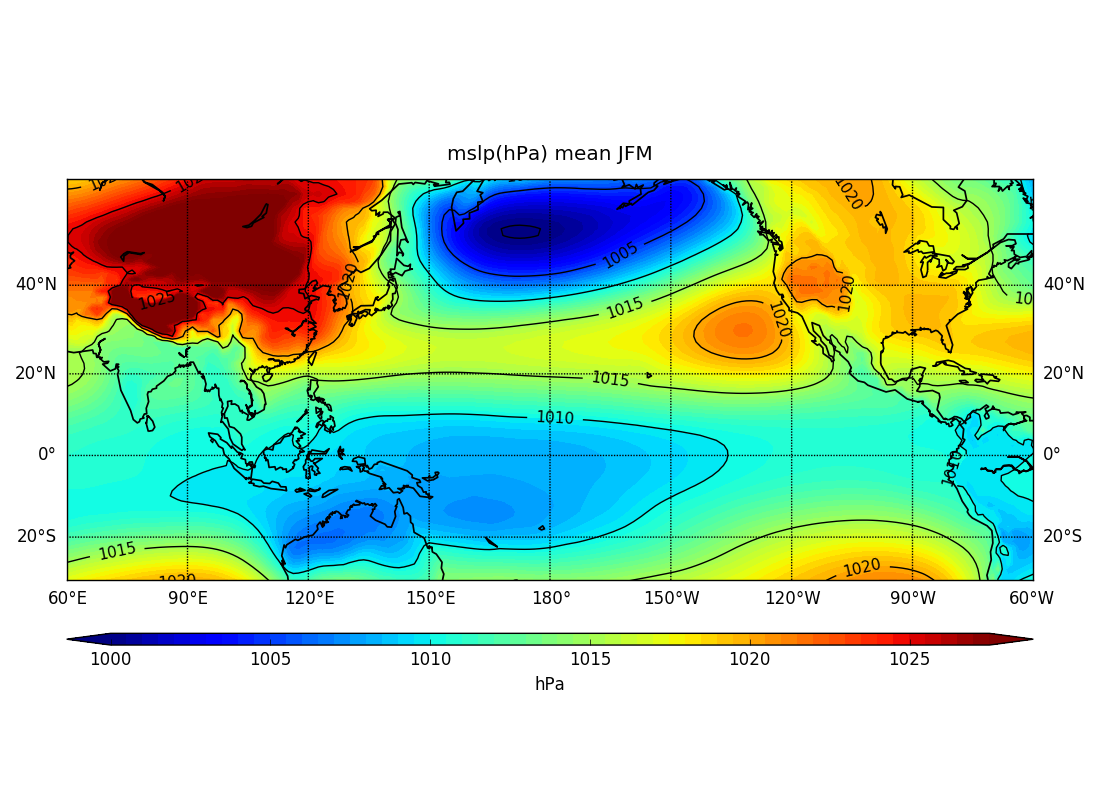
\includegraphics[width=30pc,angle=0]{Y:/Code_Data/Plots_new/Charts/mslp_JFM_mean.png}\\
% 		\noindent\includegraphics[width=30pc,angle=0]{Y:/Code_Data/Plots_new/Charts/mslp_std_JFM.png}\\
% 		\caption{MSLP climatology (a) and standard deviation (b)during the JFM season (1) and for months of JFM (2)}\label{fig:mslp_JFM}
% 	\end{figure}

%\subsection{Selection of model parameters}
%updated to 'reduced'
%The stepwise multivariate regression procedure in Matlab was given data over the training period (1958-2007). ACE-JJASO for each intensity was the predictand and the predictors were December SST in the boxes detailed above. This model found one predictor for the medium intensity storms, and none for the others. The ENPE SST region was the predictor that the model selected for the medium intensity storms, although the R2 value was only 0.133.
%Statistical relationships on maps but not in model???
%Discuss in the context of previous work
%
%%Figure 9. Sum of all tropical storms and ACE for each month over the entire period (1958-2013)
%
%% 	\begin{figure}[h]
%% 		\noindent\includegraphics[width=20pc,angle=0]{Y:/Code_Data/Plots_NCAR/MAM/Maps/regions.png}\\
%% 		\caption{Regions used in this work. The domain being examined in the recent work and regional boxes used. Note the PDO is an EOF of the SST signal from 200N}\label{fregions}
%% 	\end{figure}
%
% How many we want - cannot have too many as will be too fitted??
% Sample size of (1970-2014) 45, four predictors (10\% to avoid overfitting).
% Does the model see cross-correlation?
% Parse in different order.
% Test with different P values	

%The strongly positive correlated area for the most intense storms sits upstream of landfall, where storms will either intensify if passing over a warm SST anomaly (and other conditions are favourable), or weaken if over a cold anomaly. The climatological value of the SST in this region during SST is ....... If the SST is anomalously warm here, rapid intensification may take place and so the value of ACE at landfall will be greater. Similarly, if there is a cold anomaly, ACE will be reduced. This area is in a similar location to the negative correlation for the weakest storms and this suggests that when a warm anomaly is present, ACE for the lowest categories increase and at the same time, ACE for the most intense storms increase.
%More intense at expense of weaker? - ratios


deleted

Using GCMs, it is possible to examine how tropical cyclone activity may change in the future. The Special Report on Extreme Events from the IPCC report \citep{field2012managing} summarises, "Average tropical cyclone maximum wind speed is likely to increase, although increases may not occur in all ocean basins. It is likely that the global frequency of tropical cyclones will either decrease or remain essentially unchanged." There has also been research into changes in the tropical cyclone lifetime-maximum intensity over the past 30 years, with studies suggesting that the maximum windspeed has been migrating poleward over the past decades and will continue to do so in a warming climate \citep{kossin2014poleward} (just Atl?). As well as these changes in the activity of tropical storms in terms of frequency and distribution, each individual storm will have the potential for increased precipitation due to a simple physical relationship of the atmosphere's ability to hold more water in a warming environment. Also, the potential for sea level to continue rising is accepted, with potential increase by an additional 40cm in 21st century (IPCC, 2007). With these two well established notions, it is likely that the impact of landfalling tropical cyclones will be ameliorated. Also with an increasing population, especially around coastal areas, it is likely that for a given storm, there will be a greater population affected in the future. As discussion continues on this topic, it is still accepted that negative impacts are likely to increase, and so improvements in the forecasting of these dangerous systems and how to mitigate against their impacts is a priority.
It has been suggested that over recent decades, there has been a change in intensity distribution of hurricane intensity, with more intense storms against a background of increasing sea surface temperature \citep{webster2005changes, elsner2008increasing}. 

Observations are necessary to verify the skill of GCMs, and this can prove difficult with the relatively short ~50 years since the satellite period. The GCMs are based on physics and so what they produce may not yet have been observed in the real climate system.


There are also now a variety of reanalysis products from different agencies, for example atmosphere-only (ERA-Interim \citep{dee2011era}, JRA-55 \citep{kobayashi2015jra}, MERRA, \citep{rienecker2011merra}) as well as coupled (NCEP-CFSR \citep{saha2010ncep}). These reanalysis cover up to 55 years and newer 20th century reanalyses (e.g. \cite{compo2011twentieth}) are being created that cover the whole of the period. With a suite of these products now available, it is possible to use an ensemble approach when comparing GCMs to these 'observations'. As GCMs are being run at higher resolution, more recent reanalysis products are higher resolution than previous versions, with more complex physics, assimilation etc. 

Atlantic basin seasonal hurricane forecast - In the Atlantic, seasonal hurricane forecasts have been issued since.....initially using the quasi-biennial oscillation (QBO) and two measures of West African rainfall as predictors \citep{gray1984atlantic} - ()check this, read correct paper - also ENSO?), and updated to include conditions associated with El Ni\~{n}o-Southern Oscillation (ENSO), the Arctic Oscillation (AO) and the North Atlantic Oscillation (NAO), the Pacific-North American pattern (PNA) and the QBO \citep{klotzbach2004updated}. This showed skill, explaining about 50\% of the variance. 6-11 month forecast.

Tropical storms are the most damaging natural hazard, and in recent decades economic damage from these around the world has increased dramatically \citep{weinkle2012historical}. Rather than an attribution to climate change, it has been suggested that this increase is due to societal changes causing increased exposure \citep{pielke1998normalized}, \citep{pielke2008normalized}, \citep{weinkle2012historical}. population economic stats WPAC

Wind-driven evaporation and latent heat release within the cyclone, driving the circulation.
The cooling of these surface waters limit the intensification... etc. decreases total heat flux (latent plus sensible)

SST decreased reduces the heat and moisture fluxes.
The tropical cyclone gets its energy from the underlying ocean, through latent heating and the idea of a Carnot engine (ref). 

Aircraft are used to observe typhoons in the United States and Taiwan. In Japan it was done just once as an experiment 8 years ago since continuous observation by the US military ended in 1987.

Tropical cyclones are one of the most devastating natural hazards, causing damage from strong winds, precipitation (freshwater flooding) and storm surge. As tropical cyclones make landfall in coastal areas, which are becoming increasingly more populated, the damage caused by such systems is becoming increasingly costly.  Current state-of-the-art global climate models are capable of simulating tropical-cyclone-like vortices, and are valuable tools in predicting this phenomena, although they have limitations, for example in simulating intensity.

Current CMIP5 models assessed in the AR5 have a vertical resolution in the atmosphere of 20-50 levels \citep{climodaus}. 
Climate model resolution is also restricted by computing power, as generally increasing the resolution of a model by a factor of two requires ten times as much computing power.

A reanalysis integrates observations with a general circulation model to produce a temporally and spatially consistent synthesis of variables not easily observed. They contain data at grid points around the globe, making for ease of comparability to GCM data, and are a a close representation to the past due to the constraint on the model evolution by the observations. Although these datasets are not exact observations, due to the nature of errors in the GCM as well as the assimilated observations, they provide a best estimate of the variables and are used to explore GCMs. Tropical-storm like vortices are simulated in these models, although large differences in frequency, and distribution are apparent \citep{murakami2014tropical}.

The movement of the tropical cyclone is largely controlled by the large-scale atmospheric pattern (ref), like it is an enclosed system moving in a large scale flow. Flow plus beta drift.

Internal dynamics and external forcing.
Ocean and atmosphere can aid generate, maintain, dissipate storms. Variability depending on combination of factors.

Talk about storm being carried by the environment. Deep layer mean (DLM) steering flow approximates the TC motion.
However, TCs can depart from this \citep{galarneau2013diagnosing}. TC motion is primarily driven by environmental flow \citep{chan1982tropical} cite more Holland and Chan.

'Hurricane intensity predictions (as well as corresponding track forecast) could be significantly affected by the improved parametrisation of the air-sea momentum flux at high wind speeds \citep{moon2004effect}. 

Predictability of tropical storm activity comes from the oceanic thermodynamic conditions sea surface temperature, which is a source of memory and large-scale atmospheric patterns

In recent years, the forecasting of tropical cyclone tracks has improved, although tropical cyclone intensity forecasts are still a major challenge. I aim to examine the impact of the ocean on tropical cyclone activity and the potential predictability that representing both systems in a forecast offer.

Patterns in atmosphere and oceanic environments.
Introduce the fact that large-scale patterns cause / affect variability. 

MJO eastwards propagating active and suppressed convection, 30-90 days.
Although Harr (2006) showed that MJO influence can be overriden by other factors, as temporal clustering related to MJO phase is not exhibited in every case. Scale interaction if the most critical function for summertime climate variability in the WNP \citep{kim2008systematic}.
\citep{liu2008interdecadal}- found significant interdecadal variation expressed by three major modes.  - PDO in modes of variability section

Genesis position is very important in defining the clusters \citep{CamargoRobertsonGaffneyEtAl2007}
. Track length important for intensity, with longer-living  (El Ni\~{n}o ) reaching higher intensities, although can be affected by land, e.g. passing over Philippines \citep{CamargoRobertsonGaffneyEtAl2007}. Camargo made 7 clusters, 51\% of all cyclones make landfall, but this varies between 7\% and 85\% between clusters. Alongside spatial differences, there is a defined temporal difference, seasonal evolution and season specific. 'The mean genesis location of the TCs in the WPAC has a well-defined seasonal cycle (Chia and Ropelewski 2002, Camargo 2005), with average latitude reaching northernmost position in August and equatorward in February. Because of the presence of the WPAC warm pool, the climatological SSTs in the Philippines Sea are above 26C year round and this holds for South China Sea from May to Novemberr.' Model partition according to position and shape led to high differentiation in storm intensity and seasonally between the clusters. The influence of ENSO on TC activity over the WPAC is clearly discerned in the specific clusters \citep{camargo2007cluster}.

\cite{camargo2007cluster} found a strong relationship between ace and ENSO.


Count, pressure, wind. 
However, as this is a remote sensing technique of a complex system, there are uncertainties and limitations associated with this data source

Short record - okay for looking at seasonal / interannual, but more tricky to look at decadal signals, although some studies have been done e.g.\citep{liu2008interdecadal} Inter-decadal Liu, and Ho et al 2004.
Issue of poor data quality before the satellite era, in terms of .... and spatial coverage? See Kerr 2006. Refer to observations section. 
Short historic record - we know interannual variability, but what about decadal time scales.                          Remember, I am only looking at landfalling or striking storms, so perhaps using obs pre-satellite era is less uncertain?


Climate prediction through dynamic and statistical methods has considerably improves over the past recent decades, through understanding and supercomputing \citep{zhan2012seasonal}.

remember we just want to focus on seasonal???? viyara is real time forecasting\\

the state of ocean below the surface is also important to the cyclone system, typically down to 100-200m (Emanuel 1999) 

\cite{ranger2012deep} suggested that natural variability would be the dominant driver of the level and volatility of wind-related tropical cyclone risk over the coming decade, but alongside climate change, it will be possible to experience new levels of risk within the decade. Even with this uncertainty in tropical cyclone projections, it has been shown that global damage will increase in the future. (check mendelsohn)\\

, dropsonde data - By observing the typhoon directly, it is expected to help forecast the course and intensity more accurately and reveal the mechanism that causes typhoons to develop. 

Therefore, reason for seasonal forecasts....
decision-makers, policy, general public
What kind of predictions - NWP, seasonal, climate change. Planning, mitigation, insurance etc.

The fact that climate models no good at intensity. We are not talking about NWP, where have 24h lead times etc. For NWP. see yu2013current.
NB track variation - interaction with topography (Wu and Kuo 1999), Taiwan.

Typhoon Fanapi (2010) in the WNP had a cold wake >2.5C colder than the surrounding waters \citep{mrvaljevic2013observations}. 

Sequential TCs - upwelling is negative effect, but Rossby waves are positive effect?
TC intensity controlled by dynamic and thermodynamic processes.
Talk about enthalpy and entropy?

Ocean reanalyses: OHC in ORAs is well constrained from 1993-1009 in 0-300m layer, more spread in reanalyses deepers. Marked reduction in ensemble spread of OHC trends below 300m when Argo profiling float observations became available in early 200s \citep{palmer2015ocean}.
and tropical cyclone activity is inextricably linked to the underlying ocean characteristics

With tropical storm activity inextricably linked to ocean temperature, the possible impact of rising sea surface temperatures through global warming is of great scientific and societal concern.

Annual average landfall in China is 9 \citep{xiao2013analysis}. (1949-2006). AVerage of 9 a year landfall (1951-2008) book

The preferred TC occurrence pattern in any year is largely controlled by the genesis locations and tracks of the tropical cyclones. Genesis is related to the monsoon trough and track is related to steering flow, both of which are controlled by the large-scale flow \citep{liu2008interdecadal}. - relate to landfall

The PDO index is not an average of a region, but the leading principal component of monthly sea surface temperature variability in the Pacific from 200N and so this is how I have calculated the PDO signal within the reanalysis dataset.	